\documentclass{projetofinal}
%%%%%%%%%%%%%%%%%%%%%%%%%%%%%%%%%%%%%%%%%%%%%%%%%%%%%%%%%%%%
%        P A C O T E S
%%%%%%%%%%%%%%%%%%%%%%%%%%%%%%%%%%%%%%%%%%%%%%%%%%%%%%%%%%%%
% Adicione aqui seus pacotes
\usepackage{verbatim}
\usepackage{quoting}
\usepackage{setspace} %para a ficha de catalogação
\usepackage{float}
\usepackage[alf]{abntex2cite}
\usepackage{caption}
\usepackage{listings}
\usepackage{amssymb}
\usepackage{pdfpages}

%%%%%%%%%%%%%%%%%%%%%%%%%%%%%%%%%%%%%%%%%%%%%%%%%%
% QUADROS
%%%%%%%%%%%%%%%%%%%%%%%%%%%%%%%%%%%%%%%%%%%%%%%%%
\addto\captionsbrazilian{\renewcommand{\tablename}{Quadro}}
\addto\captionsbrazilian{\renewcommand{\listtablename}{Lista de Quadros}}

%%%%%%%%%%%%%%%%%%%%%%%%%%%%%%%%%%%%%%%%%%%%%%%%%%
% FIGURAS
%%%%%%%%%%%%%%%%%%%%%%%%%%%%%%%%%%%%%%%%%%%%%%%%%
\usepackage{graphicx}
\usepackage{siunitx}
\usepackage{hyperref}
\usepackage{xcolor}
\usepackage{subfig}

\usepackage{multirow} %% para tabelas

\usepackage{array}
\usepackage{tabu}

\usepackage{ragged2e}
\usepackage{rotating}

%%%%%%%%%%%%%%%%%%%%%%%%%%%%%%%%%%%%%%%%%%%%%%%%%%%%%%%%%%%%
% Configurações para mostrar um JSON bonitinho
%%%%%%%%%%%%%%%%%%%%%%%%%%%%%%%%%%%%%%%%%%%%%%%%%%%%%%%%%%%%
\usepackage{xcolor}

\colorlet{punct}{red!60!black}
\definecolor{background}{HTML}{EEEEEE}
\definecolor{delim}{RGB}{20,105,176}
\colorlet{numb}{magenta!60!black}

\lstdefinelanguage{json}{
    basicstyle=\normalfont\ttfamily,
    numbers=left,
    numberstyle=\scriptsize,
    stepnumber=1,
    numbersep=6pt,
    showstringspaces=false,
    breaklines=true,
    frame=lines,
    backgroundcolor=\color{background},
    literate=
     *{0}{{{\color{numb}0}}}{1}
      {1}{{{\color{numb}1}}}{1}
      {2}{{{\color{numb}2}}}{1}
      {3}{{{\color{numb}3}}}{1}
      {4}{{{\color{numb}4}}}{1}
      {5}{{{\color{numb}5}}}{1}
      {6}{{{\color{numb}6}}}{1}
      {7}{{{\color{numb}7}}}{1}
      {8}{{{\color{numb}8}}}{1}
      {9}{{{\color{numb}9}}}{1}
      {:}{{{\color{punct}{:}}}}{1}
      {,}{{{\color{punct}{,}}}}{1}
      {\{}{{{\color{delim}{\{}}}}{1}
      {\}}{{{\color{delim}{\}}}}}{1}
      {[}{{{\color{delim}{[}}}}{1}
      {]}{{{\color{delim}{]}}}}{1},
}

%%%%%%%%%%%%%%%%%%%%%%%%%%%%%%%%%%%%%%%%%%%%%%%%%%%%%%%%%%%%
% Configurações personalizadas
%%%%%%%%%%%%%%%%%%%%%%%%%%%%%%%%%%%%%%%%%%%%%%%%%%%%%%%%%%%%
\DeclareCaptionFormat{citation}{%
   \ifx\captioncitation\relax\relax\else
     \captioncitation\par
   \fi
   #1#2#3\par}
   
\newcommand*\setcaptioncitation[1]{\def\captioncitation{\textit{Fonte:}~#1}}
\let\captioncitation\relax
\captionsetup{format=citation,justification=centering}

%%%%%%%%%%%%
% Apêndice
%%%%%%%%%%%%


%\renewcommand*{\sectionautorefname}{\appendixname}

%%%%%%%%%%%%%%%%%%%%%%%%%%%%%%%%%%%%%%%%%%%%%%%%%%%%%%%%%%%%
%INICIO  DO  DOCUMENTO
%%%%%%%%%%%%%%%%%%%%%%%%%%%%%%%%%%%%%%%%%%%%%%%%%%%%%%%%%%%%
\begin{document}
\bibliographystyle{abntex2-alf}
% título da tese é obrigatório
\title{ \begin{center} SAEA: Sistema de Alocação de Espaço Acadêmico \end{center} } 
% Sensoriamento Remoto: Um Estudo de Caso Com Dados do Município Campo Verde

% autor é obrigatório;
\author{David dos Santos Machado}{\chapter*{Agradecimentos}


Agradeço à Coordenadoria de Projetos de Engenharia e Arquitetura (COPEA) pela valiosa colaboração na realização deste trabalho, por meio da cessão das plantas baixas dos espaços da universidade. Essa contribuição foi fundamental para o desenvolvimento de uma interface de visualização fiel à realidade e às dimensões dos ambientes, possibilitando que o sistema proposto representasse de forma precisa as salas, mesas e auditórios disponíveis para reserva pela comunidade acadêmica. O apoio técnico e a disponibilidade da COPEA foram essenciais para garantir a qualidade e a autenticidade deste projeto, tornando possível alinhar a proposta tecnológica às características reais da infraestrutura da instituição.

Agradeço profundamente ao meu orientador, Raimundo José Macário Costa, pela dedicação, paciência e orientação ao longo do desenvolvimento deste trabalho. Sua disponibilidade para compartilhar conhecimentos, esclarecer dúvidas e oferecer direcionamentos foi essencial para que este projeto alcançasse seus objetivos. Sua postura ética, rigor acadêmico e incentivo constante contribuíram não apenas para a qualidade desta pesquisa, mas também para o meu crescimento pessoal e profissional. Agradeço por cada conselho, correção e palavra de encorajamento durante todas as etapas do processo.

\pagebreak}

% orientador é obrigatório
\advisor[Prof.]{D.Sc. Raimundo José Macário Costa}
%\advisor[Prof.]{D.Sc. André Luiz de Castro Leal \break DECOMP/UFRRJ - Orientador }{DECOMP~-~UFRRJ}

% co-orientador é opcional
%\coadvisor[]{D.Sc. Maciel Zortea \break IBM Research - Coorientador}{}

% máximo de 3 integrantes da banca (orientador e coorientador já são adicionados automaticamente)
\banca[Prof.]{D.Sc. André Luiz de Castro Leal \break DECOMP/UFRRJ}{~-~UFRRJ}
\banca[Prof.]{D.Sc. Nome professor da banca 2 \break DECOMP/UFRRJ}{~-~UFRRJ}
\banca[Prof.]{D.Sc. Nome professor da banca 3 \break DECOMP/UFRRJ}{~-~UFRRJ}
%\banca[]{Nome,~D.Sc.}{Grupo}

\location{Seropédica, Rio de Janeiro - Brasil}{}{}
\date{Outubro}{2025}% mês e ano de defesa
\maketitle % não remover

%%%%%%%%%%%%%%%%%%%%%%%%%%%%%%%%%%%%%%%%%%%%%%%%%%%%%%%%%%%%
% Inserir a ficha Catalográfica
%%%%%%%%%%%%%%%%%%%%%%%%%%%%%%%%%%%%%%%%%%%%%%%%%%%%%%%%%%%%
\clearpage\thispagestyle{empty}\addtocounter{page}{-1}  


\newpage
\null\vfill

\begin{center}
\begin{tabular}{|p{12cm}|}%{p{12cm}}
\hline
\begin{small}
\begin{verbatim}
Machado, David dos Santos 
SAEA: Sistema de Alocação de Espaço Acadêmico
Um sistema para gerencimento do uso de espaços acadêmicos.
Seroédica / David dos Santos Machado. 
Seropédica - RJ : O Autor, 2025.
xxxii, [QTD] folhas : il., fig., tab.

Trabalho de conclusão de curso (graduação) 
Universidade Federal Rural do Rio de Janeiro.
ICE. DECOMP. Sistemas de Informação, 2024.

Inclui bibliografia e glossário.

1. Sistema de Reservas
2. Gestão de Espaços

\end{verbatim}
\end{small}
\\ \hline
\end{tabular}
\end{center}

\clearpage

\startdocument%%inicia a contagem de páginas

%%%%%%%%%%%%%%%%%%%%%%%%%
% D E D I C A T Ó R I A
%%%%%%%%%%%%%%%%%%%%%%%%
\chapter*{Dedicatória}
À minha esposa,
minha companheira de todos os dias, que esteve ao meu lado em cada passo desta caminhada.

Dedico este trabalho a você, que acreditou em mim mesmo quando eu duvidei, que me ofereceu seu amor, paciência e compreensão nos momentos em que o cansaço e a incerteza pareciam maiores do que a vontade de continuar.

Você foi o meu refúgio nos dias difíceis e a minha inspiração nos dias bons. Cada gesto de apoio, cada palavra de incentivo e cada sorriso seu foram combustíveis essenciais para que eu chegasse até aqui.

Este TCC não representa apenas o encerramento de uma etapa acadêmica, mas também o símbolo de tudo o que construímos juntos — de todos os sonhos compartilhados, das renúncias silenciosas e do amor que me fortalece e me impulsiona a ser melhor a cada dia.

A você, que é o meu porto seguro e o motivo do meu esforço e da minha alegria, dedico com todo o meu amor esta conquista.
\pagebreak
%\makededicatoriapage

%%%%%%%%%%%%%%%%%%%%%%%%%%%%%
%A G R A D E C I M E N T O S
%%%%%%%%%%%%%%%%%%%%%%%%%%%%%
\chapter*{Agradecimentos}


Agradeço à Coordenadoria de Projetos de Engenharia e Arquitetura (COPEA) pela valiosa colaboração na realização deste trabalho, por meio da cessão das plantas baixas dos espaços da universidade. Essa contribuição foi fundamental para o desenvolvimento de uma interface de visualização fiel à realidade e às dimensões dos ambientes, possibilitando que o sistema proposto representasse de forma precisa as salas, mesas e auditórios disponíveis para reserva pela comunidade acadêmica. O apoio técnico e a disponibilidade da COPEA foram essenciais para garantir a qualidade e a autenticidade deste projeto, tornando possível alinhar a proposta tecnológica às características reais da infraestrutura da instituição.

Agradeço profundamente ao meu orientador, Raimundo José Macário Costa, pela dedicação, paciência e orientação ao longo do desenvolvimento deste trabalho. Sua disponibilidade para compartilhar conhecimentos, esclarecer dúvidas e oferecer direcionamentos foi essencial para que este projeto alcançasse seus objetivos. Sua postura ética, rigor acadêmico e incentivo constante contribuíram não apenas para a qualidade desta pesquisa, mas também para o meu crescimento pessoal e profissional. Agradeço por cada conselho, correção e palavra de encorajamento durante todas as etapas do processo.

\pagebreak
%\makethankspage

%%%%%%%%%%%%%%%%%%
% E P Í G R A F E
%%%%%%%%%%%%%%%%%%
\begin{epigrafe}
    \vspace*{\fill}
    \begin{flushright}
        \textit{
            “Compartilhar espaços é mais do que dividir lugares —\\
            é construir possibilidades em conjunto.”\\[0.5cm]
            — Autoria própria
        }
    \end{flushright}
    \pagebreak
\end{epigrafe}
%\epigrafepage

%%%%%%%%%%%%%%%%%%%%%%%
%R E S U M O
%%%%%%%%%%%%%%%%%%%%%%%
Este trabalho apresenta o desenvolvimento de um sistema web voltado à gestão e reserva de espaços físicos na universidade, como mesas, salas e auditórios, destinado aos integrantes da comunidade acadêmica. O sistema busca otimizar o uso dos ambientes institucionais, promovendo a organização e o compartilhamento eficiente dos recursos disponíveis.

Para garantir uma representação fiel dos espaços, a Coordenadoria de Projetos de Engenharia e Arquitetura (COPEA) colaborou com a cessão das plantas baixas oficiais, permitindo a criação de uma interface de visualização que reproduz com precisão as dimensões e a disposição real dos ambientes.

O projeto foi desenvolvido utilizando tecnologias web modernas, com foco na usabilidade, acessibilidade e integração entre usuários e infraestrutura universitária. Como resultado, obteve-se uma ferramenta intuitiva e funcional, capaz de contribuir para o aprimoramento da gestão de espaços e o fortalecimento da convivência colaborativa na comunidade acadêmica. \hfill \break

\providecommand{\keywords}[1]{\textbf{\textit{Palavras Chave---}} #1}
\noindent\keywords{Sistema de Reservas; Gestão de Espaços; Universidade; Visualização de Ambientes;}

\pagebreak
%%%%%%%%%%%%%%%%%%%%%%%%%
%A B S T R A C T
%%%%%%%%%%%%%%%%%%%%%%%%%

This work presents the development of a web-based system designed for managing and booking physical spaces at the university, such as desks, classrooms, and auditoriums, available to members of the academic community. The system aims to optimize the use of institutional facilities, promoting organization and efficient sharing of available resources.

To ensure accurate spatial representation, the Engineering and Architecture Projects Coordination (COPEA) provided the official floor plans, which enabled the creation of an interface that faithfully reproduces the real dimensions and layout of the university’s environments.

The project was developed using modern web technologies, focusing on usability, accessibility, and seamless interaction between users and the university’s infrastructure. As a result, the system offers an intuitive and effective tool that contributes to improving space management and fostering collaborative engagement within the academic community.\hfill \break

\providecommand{\keywords}[1]{\textbf{\textit{keywords---}} #1}
\noindent\keywords{Booking System; Space Management; University; Environment Visualization;}

\pagebreak
%%%%%%%%%%%%%%%%%%%%%%%%%%%%%
%   L I S T A S
%%%%%%%%%%%%%%%%%%%%%%%%%%%%%%
% Figuras
\makefigurespage

% Tabelas
\maketablespage

% Algoritmos
% \makelistingspage


% Abreviaturas (devem estar em ordem alfabética)
\makeabrevpage{\item [API] Application Programming Interface
\item [COPEA] Coordenadoria de Projetos de Engenharia e Arquitetura
\item [DTO] Data Transfer Object
\item [EF Core] Entity Framework Core
\item [JSON] JavaScript Object Notation
\item [JWT] JSON Web Token
\item [ORM] Object-Relational Mapping
\item [QR Code] Quick Response Code
\item [REST] Representational State Transfer
\item [SGBD] Sistema Gerenciador de Banco de Dados
\item [SPA] Single-Page Application
\item [SVG] Scalable Vector Graphics
\item [TCC] Trabalho de Conclusão de Curso
\item [UFRRJ] Universidade Federal Rural do Rio de Janeiro
\item [UX] User Experience
}

% Símbolos (devem estar em ordem alfabética)
%\makesymbolspage{\item [$\mu$] 


}

% Sumário 
\maketocpage

%%%%%%%%%%%%%%%%%%%%%%%%%
%   C O N T E Ú D O
%%%%%%%%%%%%%%%%%%%%%%%%%
\startcontent

\chapter{Introdução}\label{chp:INTRO}
\section{Apresentação}\label{sec:APRESENT}

Este trabalho apresenta o desenvolvimento de um sistema web destinado à reserva de mesas, salas e auditórios da universidade, permitindo que integrantes da comunidade acadêmica utilizem os espaços de forma organizada e eficiente.

\section{Motivação}\label{sec:MOTIVACAO}
%Explique por que você escolheu esse tema.
%Pode incluir problemas enfrentados atualmente (ex.: conflitos de horários, dificuldades em visualizar os espaços, ocupação inadequada).
%Relacione com benefícios potenciais.

A motivação para este estudo surge da necessidade de otimizar o uso dos espaços da universidade e facilitar o agendamento de ambientes, garantindo que a infraestrutura disponível seja utilizada de forma eficiente e transparente.

\section{Justificativa}\label{sec:Justificativa}
%Argumente por que este trabalho é relevante.
%Pode incluir impacto acadêmico, social ou tecnológico.
%Mencione como a interface baseada nas plantas baixas agrega valor.

O sistema proposto contribui para a gestão inteligente dos espaços universitários, permitindo planejamento e ocupação adequados, além de reduzir conflitos e desperdício de recursos. A utilização das plantas baixas fornecidas pela COPEA garante que a visualização seja precisa, aumentando a confiabilidade do sistema.

\section{Hipótese}\label{sec:HIPOTESE}
%Apresente uma suposição inicial sobre o resultado ou efeito do seu sistema.
%Ex.: o sistema facilitará a reserva de espaços, otimizará ocupação e reduzirá conflitos.
Hipotetiza-se que a implementação de um sistema de reservas com interface de visualização realista permitirá uma gestão mais eficiente dos espaços da universidade, promovendo organização e melhor aproveitamento da infraestrutura disponível.

\section{Objetivos}\label{sec:OBJETIVOS}

\subsection{Objetivos Gerais}\label{sec:OB_GERAIS}
% meta principal do trabalho.
Desenvolver um sistema web para reserva de mesas, salas e auditórios da universidade, com interface de visualização baseada nas plantas baixas, que otimize o uso dos espaços e facilite a organização para a comunidade acadêmica.

\subsection{Objetivos Específicos}\label{sec:OB_Específicos}
% Objetivos Específicos: etapas ou ações para atingir o objetivo geral.
bla bla bla

\begin{itemize}
\item Implementar uma interface gráfica que reproduza fielmente os espaços da universidade;
\item Permitir o agendamento e gerenciamento de reservas por membros da comunidade acadêmica;;
\item Integrar mecanismos de verificação de disponibilidade para evitar conflitos de horários;
\item Garantir usabilidade e acessibilidade na interação do usuário com o sistema.
\end{itemize}

\section{Organização do Trabalho}\label{sec:ORGANIZA}

%Explique como o TCC está estruturado, capítulo por capítulo.
%Curto parágrafo descrevendo o conteúdo de cada capítulo.
O trabalho está organizado da seguinte forma: o Capítulo 1 apresenta a introdução, contextualizando o tema, motivação, justificativa, hipótese e objetivos; o Capítulo 2 aborda a fundamentação teórica e tecnologias utilizadas; o Capítulo 3 descreve o desenvolvimento do sistema, incluindo arquitetura, interface e funcionalidades; o Capítulo 4 apresenta testes, resultados e avaliação do sistema; e, por fim, o Capítulo 5 traz as conclusões, contribuições, limitações e sugestões para trabalhos futuros.

\pagebreak
\chapter{Fundamentação Teórica}\label{chp:FUNDAMENTACAO}

Este capítulo apresenta os fundamentos teóricos e tecnológicos que embasam o desenvolvimento do sistema proposto. Inicialmente, discutem-se os conceitos de sistemas de reserva e gestão de espaços; em seguida, abordam-se as técnicas de visualização de ambientes, as tecnologias de desenvolvimento web e os princípios de experiência do usuário; por fim, apresentam-se estudos de caso e trabalhos relacionados que contextualizam a solução desenvolvida.

%Cada seção deve começar com uma definição ou conceito e terminar mostrando como isso se relaciona com o seu sistema.

%Sempre que possível, inclua referências acadêmicas recentes para fortalecer a fundamentação.

%Use figuras ou exemplos (como screenshots ou esquemas de plantas baixas) para ilustrar conceitos importantes.

\section{Sistemas de Reserva e Gestão de Espaços}\label{sec:sistemasDeReservaEGestaoDeEspacos}

% Conceitos de sistemas de reservas de ambientes.
% Tipos de sistemas (universidades, empresas, coworkings).
% Benefícios para gestão de recursos e otimização de uso.
% Exemplos de trabalhos acadêmicos relacionados.

Sistemas de reserva são aplicações destinadas a mediar o acesso compartilhado a recursos de disponibilidade limitada, coordenando a demanda de múltiplos usuários ao longo do tempo e evitando a sobreposição de uso. % TODO: \cite{ref-sistemas-reserva}
No contexto da gestão de espaços físicos, tais sistemas permitem que ambientes como salas, mesas e auditórios sejam agendados de forma organizada, substituindo controles manuais — como planilhas, livros de registro ou comunicação informal — por um processo centralizado, rastreável e acessível remotamente.

Esse tipo de solução é encontrado em contextos diversos, como espaços de trabalho compartilhado (\textit{coworkings}), empresas que gerenciam salas de reunião e instituições de ensino que administram laboratórios e ambientes de estudo. Em todos esses casos, os benefícios são semelhantes: melhor aproveitamento da infraestrutura disponível, redução de conflitos de agendamento, transparência quanto à ocupação e obtenção de dados que apoiam o planejamento do uso dos espaços. % TODO: \cite{ref-gestao-espacos}

No ambiente acadêmico, a gestão de espaços apresenta particularidades relevantes, como a existência de diferentes perfis de usuário, a necessidade de aprovação por responsáveis e a alta rotatividade de uso ao longo do dia. O sistema proposto neste trabalho insere-se nesse contexto, oferecendo um mecanismo de reserva \textit{self-service} associado a fluxos de aprovação e a políticas de uso que visam coibir o desperdício de recursos.

\section{Visualização de ambientes}\label{sec:visualizacaoDeAmbientes}

%Técnicas de visualização de plantas baixas.
%Modelos 2D e 3D para interfaces de usuários.
%Softwares e ferramentas comuns (ex.: CAD, Google Indoor Maps).
%Importância da fidelidade da visualização para a experiência do usuário.

A visualização de ambientes diz respeito às técnicas empregadas para representar graficamente espaços físicos em interfaces digitais, de modo que o usuário compreenda a disposição e a ocupação dos recursos. As representações podem ser bidimensionais (2D), como plantas baixas e mapas esquemáticos, ou tridimensionais (3D), como modelos volumétricos e ambientes navegáveis. As representações 2D destacam-se pela clareza e pelo baixo custo computacional, sendo especialmente adequadas à visão geral de um pavimento. % TODO: \cite{ref-visualizacao}

Plantas baixas são tradicionalmente produzidas em ferramentas de desenho assistido por computador (\textit{Computer-Aided Design} — CAD) e em editores gráficos vetoriais. Soluções de mapeamento de ambientes internos, como serviços de mapas em espaços fechados, evidenciam o valor de representar fielmente a estrutura real para orientar o usuário. A fidelidade da visualização é, portanto, um fator determinante da experiência: quanto mais a representação corresponde ao ambiente real, maior a confiança do usuário e menor o esforço cognitivo necessário para localizar e selecionar um recurso. % TODO: \cite{ref-fidelidade-visual}

Neste trabalho, a visualização foi construída a partir das plantas baixas oficiais dos ambientes, redesenhadas e exportadas em formato vetorial, o que garante precisão dimensional e permite a interação direta sobre a representação dos espaços, conforme detalhado no Capítulo~\ref{chp:METODOLOGIA}.

\section{Tecnologias de Desenvolvimento Web}\label{sec:tecnologiasDesenvolvimentoWeb}
%Tecnologias utilizadas para o sistema (front-end, back-end, frameworks).
%Integração com bancos de dados para reservas.
%Padrões de usabilidade e acessibilidade em aplicações web.

Aplicações web modernas são comumente estruturadas segundo o modelo cliente-servidor, no qual a interface executada no navegador (\textit{front-end}) comunica-se com um serviço de retaguarda (\textit{back-end}) responsável pela lógica de negócio e pela persistência dos dados. Essa comunicação costuma ocorrer por meio de APIs no estilo REST, que padronizam o acesso aos recursos e favorecem o desacoplamento entre as camadas. % TODO: \cite{ref-rest}

No \textit{front-end}, \textit{frameworks} para a construção de aplicações de página única (SPA) permitem interfaces ricas e responsivas, nas quais a navegação ocorre sem recarregamentos completos da página. No \textit{back-end}, plataformas maduras oferecem recursos para a construção de serviços seguros e de alto desempenho, incluindo autenticação, autorização e validação de dados. A persistência, por sua vez, apoia-se frequentemente em SGBDs relacionais, acessados por meio de bibliotecas de mapeamento objeto-relacional (ORM), que reduzem a distância entre o modelo de objetos da aplicação e o modelo de tabelas do banco de dados. % TODO: \cite{ref-orm}

Além da funcionalidade, aplicações web devem observar padrões de usabilidade e de acessibilidade, garantindo que a interface seja utilizável por pessoas com diferentes capacidades e em diferentes dispositivos. As tecnologias específicas adotadas neste trabalho e as justificativas para sua escolha são apresentadas no Capítulo~\ref{chp:METODOLOGIA}.

\section{Experiência do Usuário (UX)}\label{sec:ux}
%Princípios de design de interfaces para sistemas de reserva.
%Métodos para tornar o sistema intuitivo e eficiente.
%Pesquisas que mostram impacto da interface na satisfação do usuário.

A experiência do usuário (\textit{User Experience} — UX) abrange o conjunto de percepções e respostas resultantes da interação de uma pessoa com um sistema, englobando aspectos como facilidade de uso, eficiência, clareza e satisfação. % TODO: \cite{ref-ux}
O projeto de interfaces orientado à UX apoia-se em princípios como consistência, prevenção de erros, retorno imediato às ações do usuário e redução da carga cognitiva, de modo que o sistema seja intuitivo e demande pouco esforço de aprendizagem.

Em sistemas de reserva, esses princípios traduzem-se em fluxos objetivos para consultar disponibilidade e concretizar um agendamento, em mensagens claras diante de restrições ou erros e em uma representação visual que facilite a localização dos recursos. A literatura aponta que a qualidade da interface influencia diretamente a satisfação e a adesão dos usuários, impactando a efetividade da solução. % TODO: \cite{ref-ux-satisfacao}
Esses fundamentos orientaram as decisões de projeto da interface deste trabalho, especialmente no que se refere à visualização interativa das plantas baixas e ao suporte a múltiplos idiomas.

\section{Estudos de Casos e Trabalhos Relacionados}\label{sec:trabsrelacionados}
%Apresentar sistemas similares implementados em outras universidades ou empresas.
%Comparar soluções existentes com a proposta do seu sistema.
%Identificar lacunas que o seu trabalho pretende preencher.

Diversas soluções abordam a reserva e a gestão de espaços, desde plataformas comerciais de agendamento de salas até sistemas desenvolvidos no âmbito acadêmico. % TODO: \cite{ref-trabalho-relacionado-1, ref-trabalho-relacionado-2}
De modo geral, essas soluções contemplam o cadastro de recursos, a consulta de disponibilidade e o registro de reservas; contudo, muitas apresentam a disponibilidade por meio de listas ou grades de horário, sem uma representação espacial fiel do ambiente.

A comparação entre as soluções existentes e a proposta deste trabalho é sintetizada no Quadro~\ref{tab:comparativo-trabalhos}. % TODO: preencher o quadro comparativo com os trabalhos relacionados selecionados.
A principal lacuna identificada refere-se à combinação, em uma única solução voltada ao contexto acadêmico, de visualização interativa baseada nas plantas baixas reais, fluxo de aprovação por gestores e política de penalidades por não comparecimento — conjunto de características que orienta a contribuição do presente trabalho.

\begin{table}[H]
  \centering
  \caption{Comparativo entre trabalhos relacionados e a proposta}
  \label{tab:comparativo-trabalhos}
  \begin{tabular}{|p{4cm}|p{3.2cm}|p{2.4cm}|p{2.4cm}|}
    \hline
    \textbf{Solução} & \textbf{Visualização fiel} & \textbf{Aprovação} & \textbf{Penalidades} \\
    \hline
    Trabalho relacionado 1 & --- & --- & --- \\
    \hline
    Trabalho relacionado 2 & --- & --- & --- \\
    \hline
    Proposta (este trabalho) & Sim & Sim & Sim \\
    \hline
    % TODO: ajustar as linhas conforme os trabalhos relacionados selecionados.
  \end{tabular}\\
  {\footnotesize Fonte: Autoria própria.}
\end{table}

\pagebreak


\chapter{Metodologia}\label{chp:AP_Results}

%Use diagramas de arquitetura (ex.: fluxos de dados, containers Docker).

%Inclua tabelas de requisitos e exemplos de telas para ilustrar a metodologia.

%Sempre explique por que escolheu cada tecnologia, mostrando alinhamento com os objetivos do sistema.

\section{Tipo de Pesquisa}\label{sec:tipoPesquisa}
%Explique se o trabalho é aplicado, experimental ou de desenvolvimento tecnológico.

%Exemplo: pesquisa aplicada com desenvolvimento de protótipo de sistema para reserva de ambientes acadêmicos.


\section{Levantamento de Requisitos}\label{sec:requisitos}
%Descreva como você identificou as necessidades da comunidade acadêmica.
%Métodos: entrevistas, questionários, observação, análise de sistemas existentes.
%Liste os requisitos funcionais e não funcionais do sistema.
Para identificar as necessidades e expectativas dos usuários do sistema de reservas, foi elaborado um questionário direcionado aos funcionários da biblioteca, responsáveis pela gestão dos espaços acadêmicos. O objetivo é coletar informações sobre o uso atual das salas, mesas e auditórios, dificuldades enfrentadas no processo de reserva e funcionalidades desejadas para o novo sistema. O questionário completo encontra-se disponível no \hyperref[apendice:entrevistas]{Apêndice A}.

O questionário combina perguntas objetivas e abertas, permitindo tanto a obtenção de dados quantitativos, como frequência de uso e problemas mais comuns, quanto dados qualitativos, como sugestões de melhorias e funcionalidades essenciais. Entre os tópicos abordados, destacam-se:
\begin{itemize}
  \item Uso atual dos espaços: frequência de reservas, problemas encontrados, sistemas atualmente utilizados.
  \item Funcionalidades desejadas: prioridades na gestão de reservas, tipos de visualização dos ambientes e recursos que devem ser disponibilizados.
  \item Usabilidade e experiência do usuário: facilidade de uso, informações essenciais na interface e percepção sobre a redução de conflitos.
  \item Sugestões e melhorias: opiniões abertas sobre funcionalidades essenciais e formas de otimizar o sistema.
\end{itemize}

A aplicação do questionário tem o potencial de identificar requisitos funcionais e não funcionais do sistema, bem como alinhar o desenvolvimento da interface e das funcionalidades às reais necessidades da comunidade acadêmica. Os dados coletados serão analisados e utilizados como base para o projeto do sistema, garantindo que a solução proposta seja eficiente, prática e adequada ao contexto da universidade.

\section{Arquitetura do Sistema}\label{sec:arquitetura}
%Apresente diagrama de arquitetura (Front-end, Back-end, Banco de dados).
%Explique a escolha de tecnologias: Angular (front-end), PHP (back-end), MySQL (banco de dados), Docker (containerização).
%Mostre como cada componente se comunica (ex.: Angular → PHP → MySQL).

\section{Desenvolvimento do Sistema}\label{sec:desenvolvimento}
\subsection{Front-end (Angular)}\label{subsec:angular}
%Componentes, rotas, interface de visualização das plantas baixas.
%Interação com o usuário (reserva de mesas, salas, auditorios).

\subsection{Back-end (.NET)}\label{subsec:dotnet}
%APIs e endpoints para gerenciamento de reservas.
%Validação de dados, autenticação de usuários.

\subsection{Banco de Dados (MySQL)}\label{subsec:mysql}
%Estrutura de tabelas, relacionamentos, integridade de dados.

\subsection{Docker}\label{subsec:docker}
%Containerização do ambiente de desenvolvimento e produção.
%Benefícios de portabilidade e padronização.


\section{Interface de Visualização dos Espaços}\label{sec:interface}
%Explique como você representou as plantas baixas de forma fiel.
%Métodos de renderização (2D/3D, grid, mapas interativos).
%Integração entre front-end e dados do banco de dados.

\subsection{Sub-tópico}\label{subsec:landsat}

\section{Testes e Validação}\label{sec:testesValidacao}
%Testes funcionais: reserva de mesas, salas e auditorios.
%Testes de usabilidade: interface intuitiva e responsiva.
%Testes de integração: front-end, back-end e banco funcionando corretamente.

\subsection{Sub-tópico}\label{subsec:landsat}

\section{Ferramentas e Ambientes de Desenvolvimento}\label{sec:ferramentas}
%Softwares utilizados (VS Code, MySQL Workbench, Docker Desktop, Git, etc.).

%Ambientes (desenvolvimento local, testes, produção).

\pagebreak


\chapter{Resultados}\label{chp:RESULTADOS}

Este capítulo apresenta os resultados obtidos com o desenvolvimento do sistema, descrevendo a implementação realizada, demonstrando as principais funcionalidades por meio de telas da aplicação, relatando os testes conduzidos e, por fim, confrontando os resultados com os objetivos estabelecidos no Capítulo~\ref{chp:INTRO}.

\section{Implementação do Sistema}\label{sec:implementacao}
% Descreva aqui o sistema desenvolvido, módulos principais e funcionalidades.
% Inclua imagens ou diagramas de telas se necessário.

O sistema foi implementado conforme a arquitetura descrita no Capítulo~\ref{chp:METODOLOGIA}, resultando em uma aplicação \textit{web} funcional composta por uma interface Angular e uma API em ASP.NET Core apoiada em banco de dados SQL Server. A solução contempla os módulos de autenticação, consulta de disponibilidade e visualização de plantas baixas, reserva de recursos, aprovação e moderação por gestores, bloqueios administrativos, gestão de usuários e acompanhamento por meio de painel (\textit{dashboard}) e histórico.

O acesso ao sistema é diferenciado por perfil de usuário. Os membros da comunidade acadêmica realizam reservas de forma autônoma; os gestores de pavilhão moderam as solicitações e administram bloqueios; e os administradores gerenciam usuários e a configuração geral. A tela inicial de autenticação é apresentada na Figura~\ref{fig:tela-login}.

\begin{figure}[H]
  \centering
  \framebox[0.7\textwidth]{\rule{0pt}{7cm}}% PLACEHOLDER — substituir pela linha \includegraphics abaixo
  % \includegraphics[width=0.7\textwidth]{imagens/resultados/tela-login.png}
  \caption{Tela de autenticação do sistema.}
  \label{fig:tela-login}\\
  {\footnotesize Fonte: Autoria própria.}
\end{figure}

\section{Demonstração das Funcionalidades}\label{sec:demonstracao}
% Mostre como o sistema funciona na prática.
% Exemplos: reserva de mesas, salas e auditórios.
% Inclua figuras, fluxogramas ou telas da interface.

\subsection{Consulta de disponibilidade e reserva}\label{subsec:demo-reserva}

O fluxo central do sistema é a reserva de recursos. Após autenticar-se, o usuário seleciona o pavimento, a data e o intervalo de horário desejados e visualiza, sobre a planta baixa, a ocupação em tempo real: os recursos disponíveis são destacados em verde e os indisponíveis são atenuados. A Figura~\ref{fig:mapa-consulta} apresenta a tela de consulta com a planta baixa de um pavimento.

\begin{figure}[H]
  \centering
  \framebox[0.9\textwidth]{\rule{0pt}{8cm}}% PLACEHOLDER — substituir pela linha \includegraphics abaixo
  % \includegraphics[width=0.9\textwidth]{imagens/resultados/mapa-consulta.png}
  \caption{Consulta de disponibilidade sobre a planta baixa do pavimento.}
  \label{fig:mapa-consulta}\\
  {\footnotesize Fonte: Autoria própria.}
\end{figure}

Ao selecionar um recurso disponível, o sistema exibe um resumo da reserva para confirmação, contendo a identificação do recurso, a data, a capacidade e as orientações de uso, incluindo as consequências do não comparecimento. A Figura~\ref{fig:modal-confirmacao} ilustra essa etapa.

\begin{figure}[H]
  \centering
  \framebox[0.6\textwidth]{\rule{0pt}{6cm}}% PLACEHOLDER — substituir pela linha \includegraphics abaixo
  % \includegraphics[width=0.6\textwidth]{imagens/resultados/modal-confirmacao.png}
  \caption{Confirmação de reserva de um recurso.}
  \label{fig:modal-confirmacao}\\
  {\footnotesize Fonte: Autoria própria.}
\end{figure}

\subsection{Acompanhamento das reservas e check-in}\label{subsec:demo-minhas-reservas}

Após efetuar uma reserva, o usuário acompanha sua situação na área de reservas, na qual é possível cancelar solicitações e realizar o \textit{check-in} por meio de \textit{QR Code} dentro da janela de tolerância. A Figura~\ref{fig:minhas-reservas} apresenta essa listagem.

\begin{figure}[H]
  \centering
  \framebox[0.9\textwidth]{\rule{0pt}{6cm}}% PLACEHOLDER — substituir pela linha \includegraphics abaixo
  % \includegraphics[width=0.9\textwidth]{imagens/resultados/minhas-reservas.png}
  \caption{Acompanhamento das reservas do usuário.}
  \label{fig:minhas-reservas}\\
  {\footnotesize Fonte: Autoria própria.}
\end{figure}

\subsection{Aprovação e moderação pelo gestor}\label{subsec:demo-aprovacao}

As reservas seguem um fluxo de aprovação sob responsabilidade do gestor do pavilhão, que pode aprovar ou rejeitar solicitações e, quando necessário, revogar reservas já aprovadas. A Figura~\ref{fig:aprovacoes} apresenta a tela de moderação.

\begin{figure}[H]
  \centering
  \framebox[0.9\textwidth]{\rule{0pt}{6cm}}% PLACEHOLDER — substituir pela linha \includegraphics abaixo
  % \includegraphics[width=0.9\textwidth]{imagens/resultados/aprovacoes.png}
  \caption{Fila de aprovação de reservas do gestor.}
  \label{fig:aprovacoes}\\
  {\footnotesize Fonte: Autoria própria.}
\end{figure}

\subsection{Painel e histórico}\label{subsec:demo-dashboard}

O sistema disponibiliza ainda um painel com indicadores de uso dos espaços e um histórico das reservas, apoiando o acompanhamento gerencial. A Figura~\ref{fig:dashboard} apresenta o painel.

\begin{figure}[H]
  \centering
  \framebox[0.9\textwidth]{\rule{0pt}{7cm}}% PLACEHOLDER — substituir pela linha \includegraphics abaixo
  % \includegraphics[width=0.9\textwidth]{imagens/resultados/dashboard.png}
  \caption{Painel de indicadores de uso dos espaços.}
  \label{fig:dashboard}\\
  {\footnotesize Fonte: Autoria própria.}
\end{figure}

\section{Testes e Validação}\label{sec:testes}
% Resultados dos testes funcionais e de usabilidade.
% Inclua métricas, tabelas ou gráficos de desempenho e satisfação dos usuários.

A validação do sistema foi conduzida conforme o planejamento descrito na Seção~\ref{sec:testesValidacao}. Os testes funcionais verificaram o comportamento das principais operações, incluindo os fluxos de exceção. O Quadro~\ref{quadro:testes-funcionais} sintetiza os casos de teste executados e seus resultados.

\begin{table}[H]
  \centering
  \caption{Casos de teste funcionais e resultados.}
  \label{quadro:testes-funcionais}
  \begin{tabular}{|p{1.6cm}|p{6cm}|p{4.5cm}|}
    \hline
    \textbf{Caso} & \textbf{Cenário} & \textbf{Resultado esperado} \\
    \hline
    CT-01 & Autenticação com credenciais válidas & Acesso concedido \\
    \hline
    CT-02 & Reserva de recurso disponível & Reserva registrada como pendente \\
    \hline
    CT-03 & Reserva em horário já ocupado & Operação bloqueada \\
    \hline
    CT-04 & Aprovação de reserva pelo gestor & Reserva aprovada \\
    \hline
    CT-05 & \textit{Check-in} dentro da janela de tolerância & Reserva em andamento \\
    \hline
    % TODO: complementar com os demais casos de teste executados.
  \end{tabular}\\
  {\footnotesize Fonte: Autoria própria.}
\end{table}

Os testes de usabilidade avaliaram a clareza e a facilidade de uso da interface junto aos usuários. Os indicadores coletados e a percepção dos participantes são apresentados no Quadro~\ref{quadro:testes-usabilidade}. % TODO: preencher com os dados obtidos após a aplicação dos testes de usabilidade.

\begin{table}[H]
  \centering
  \caption{Resultados dos testes de usabilidade.}
  \label{quadro:testes-usabilidade}
  \begin{tabular}{|p{8cm}|p{3.5cm}|}
    \hline
    \textbf{Critério avaliado} & \textbf{Resultado} \\
    \hline
    Facilidade de uso & --- \\
    \hline
    Clareza da visualização das plantas baixas & --- \\
    \hline
    Percepção de redução de conflitos & --- \\
    \hline
    Satisfação geral & --- \\
    \hline
  \end{tabular}\\
  {\footnotesize Fonte: Autoria própria.}
\end{table}

\section{Comparação com os Objetivos}\label{sec:comparacao}
% Explique como o sistema atingiu o objetivo geral e os objetivos específicos.
% Destaque o que foi alcançado.

Confrontando os resultados com os objetivos específicos definidos na Seção~\ref{sec:OB_Específicos}, verifica-se que o sistema desenvolvido atendeu às metas estabelecidas. O Quadro~\ref{quadro:objetivos} relaciona cada objetivo específico ao respectivo resultado alcançado.

\begin{table}[H]
  \centering
  \caption{Relação entre objetivos específicos e resultados alcançados.}
  \label{quadro:objetivos}
  \begin{tabular}{|p{7.5cm}|p{4cm}|}
    \hline
    \textbf{Objetivo específico} & \textbf{Situação} \\
    \hline
    Modelar o domínio de reservas de espaços acadêmicos & Atendido \\
    \hline
    Desenvolver interface com visualização das plantas baixas & Atendido \\
    \hline
    Permitir o agendamento e o gerenciamento de reservas & Atendido \\
    \hline
    Implementar a verificação de disponibilidade & Atendido \\
    \hline
    Disponibilizar fluxo de aprovação e moderação & Atendido \\
    \hline
    Prover \textit{check-in} e política de penalidades & Atendido \\
    \hline
    Garantir usabilidade, acessibilidade e múltiplos idiomas & Atendido \\
    \hline
  \end{tabular}\\
  {\footnotesize Fonte: Autoria própria.}
\end{table}

\section{Discussão dos Resultados}\label{sec:discussao}
% Comente pontos fortes, limitações e melhorias futuras.
% Analise os resultados em relação ao contexto acadêmico e tecnológico.

Entre os pontos fortes do sistema destaca-se a visualização interativa baseada nas plantas baixas reais, que aproxima a experiência digital do ambiente físico e reduz o esforço do usuário para localizar e reservar um recurso. A adoção de uma arquitetura em camadas favoreceu a organização e a manutenção do código, enquanto o fluxo de aprovação e a política de penalidades contribuem para o uso responsável dos espaços.

Como limitações, observa-se que a fidelidade da visualização depende da disponibilidade e da atualização das plantas baixas oficiais, e que a validação com usuários, embora planejada, ainda demanda ampliação para conclusões mais abrangentes. Tais limitações, contudo, não comprometem os resultados obtidos e apontam caminhos para o aprimoramento da solução, discutidos no Capítulo~\ref{chp:CONCLUSAO}.
\pagebreak
\chapter{Considerações Finais}\label{chp:CONCLUSAO}

Este trabalho teve como objetivo o desenvolvimento de um sistema \textit{web} para a reserva de mesas, salas e auditórios da universidade, dotado de uma interface de visualização baseada nas plantas baixas reais dos ambientes. A partir do levantamento das necessidades da comunidade acadêmica e do estudo das tecnologias pertinentes, foi projetada e implementada uma solução funcional, organizada em uma arquitetura em camadas e apoiada em tecnologias web consolidadas.

Os resultados apresentados no Capítulo~\ref{chp:RESULTADOS} indicam que o sistema atingiu os objetivos propostos: a reserva de recursos pode ser realizada de forma autônoma e visual, a disponibilidade é verificada de modo a evitar conflitos, e o fluxo de aprovação, associado à política de penalidades por não comparecimento, promove o uso responsável dos espaços. A representação fiel dos ambientes, viabilizada pelas plantas baixas cedidas pela COPEA e pelo processo de vetorização e normalização dos desenhos, constitui o principal diferencial da solução, aproximando a experiência digital do ambiente físico.

Como contribuição, o trabalho oferece uma alternativa concreta para a gestão de espaços acadêmicos, com potencial de reduzir conflitos, otimizar a ocupação da infraestrutura e aumentar a transparência do processo de reserva. Confirma-se, assim, a hipótese de que um sistema de reservas com interface de visualização realista favorece uma gestão mais eficiente dos espaços da universidade.

\section{Trabalhos Futuros}\label{sec:trab_futuros}

A partir dos resultados obtidos e das limitações identificadas, apontam-se as seguintes possibilidades de trabalhos futuros:

\begin{itemize}
  \item Ampliar a validação com usuários, por meio de testes de usabilidade em maior escala, a fim de consolidar as conclusões sobre a experiência de uso;
  \item Estender a cobertura do sistema a outros pavilhões e edifícios da universidade, incorporando novas plantas baixas;
  \item Automatizar a etapa de normalização dos vetores, reduzindo o esforço manual na preparação de novas plantas;
  \item Desenvolver uma versão para dispositivos móveis ou um aplicativo dedicado, ampliando a acessibilidade da solução;
  \item Incorporar recursos de análise de dados e relatórios gerenciais mais elaborados, apoiando a tomada de decisão sobre a utilização dos espaços;
  \item Integrar o sistema a serviços institucionais de autenticação, unificando o acesso com as credenciais já utilizadas pela comunidade acadêmica.
\end{itemize}

\pagebreak


\pagebreak

%%%%%%%%%%%%%%%%%%%%%%%%%%%%%
% B I B L I O G R A F I A
%%%%%%%%%%%%%%%%%%%%%%%%%%%%%%
% Retirar esta parte se o trabalho não tiver bibliografia
\makebibspage{abnt}{elementos-postextuais/referencias}


%%%%%%%%%%%%%%%%%%%%%%%
% A P E N D I C E
%%%%%%%%%%%%%%%%%%%%%%%%
% Retirar esta parte se o trabalho não tiver anexos
\appendix
\chapter{Formulário para Entrevista Inicial}\label{apendice:entrevistas}

Segue o questionário utilizado para levantamento de requisitos do sistema de reservas de mesas, salas e auditórios, aplicado aos funcionários da biblioteca:


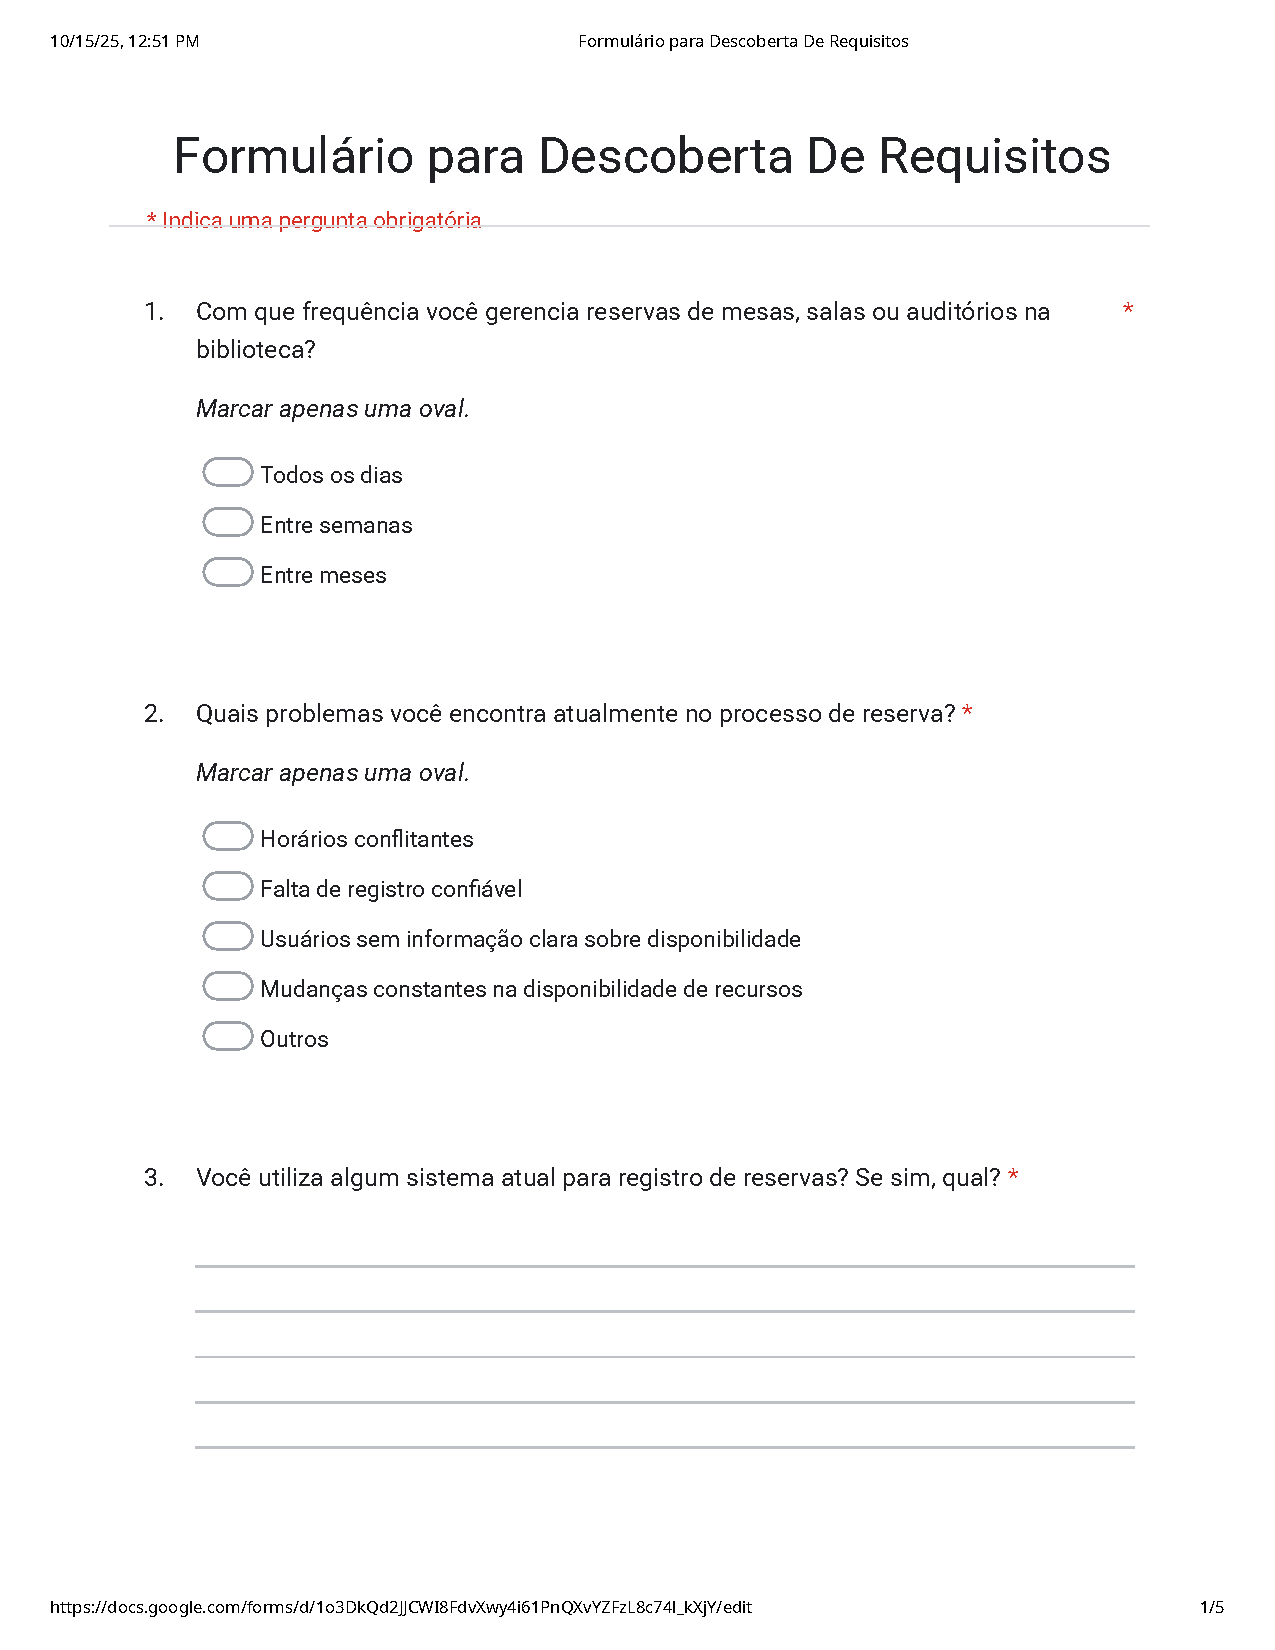
\includepdf[pages={1,2,3}]{anexos/TCC_DAVID_Formulario.pdf}

\end{document}